\subsection{General Unsupervised Sequence Model}
 \frame[t] {%slide 9
 \frametitle{Big Picture}
 Can we learn a joint distribution of over sequences of unbounded length given a single training sequence? (!!!) \newline
 
\begin{itemize}
\item Obviously not without strong regularization.  
\end{itemize}

 
 \begin{block}{Proposal}
\begin{itemize}
\item Build hierarchical model that ties together conditional distributions in ``natural'' way
\item What would such a model look like?
\end{itemize}
\end{block}
%Let $G_{[\ubf]}$ be the conditional distribution over $\{0,1\}$, conditioned on the binary sequence $\ubf$
}

 \frame[t] {%slide 8
 \frametitle{Regularized Joint Model for Discrete Data}
 Let $\GG = \{G_{[\ubf]}\}, \forall \ubf \in \Sigma^+$ be all conditional distributions over a finite alphabet and $\xbf = x_1, x_2, \ldots, x_n$ be a sequence of discrete observations
\begin{eqnarray*}
P(\xbf,\GG) &=& P(\GG)P(\xbf|\GG) \nonumber \\
P(\xbf,\GG) &=& P(\GG)\prod_{i=0}^{|\xbf|-1}G_{\xbf_{1:i}}(\xbf_{i+1})
\end{eqnarray*}
Where, expanding $P(\xbf|\GG)$ to make it clearer
\begin{align}
P(\xbf|\GG) = G_{[]}(x_{1})G_{x_1}(x_{2})G_{\xbf_{1:2}}(x_{3})\cdots G_{\xbf_{1:(|\xbf|-1)}}(x_{|\xbf|})  \nonumber 
\end{align}
Note that this is the ``joint''\footnote{$P(x_1,\ldots,x_i|\theta) = P(x_1|\theta) P(x_2 | x_1, \theta) P(x_3 | x_1,x_2, \theta) \cdots P(x_i | \xbf_{1:(i-1)}, \theta)$} distribution of $\xbf$ and $P(\GG)$ directly regularizes the joint distribution itself.

 }


  \frame[t] {%slide 27
 \frametitle{The Corresponding Graphical Model}
 \begin{figure}[htbp]
\begin{center}
%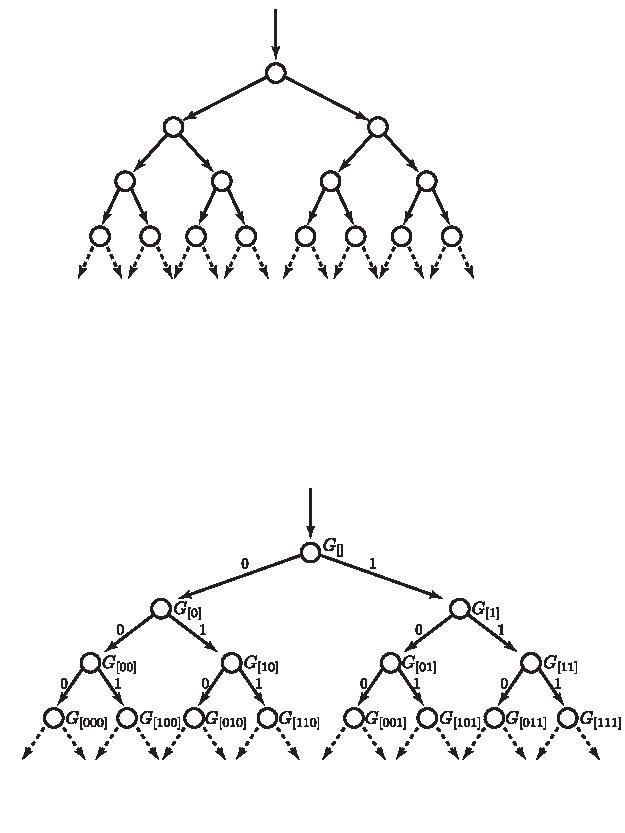
\includegraphics[trim = 4cm 8cm 4cm 8cm, clip, width=5cm]{jtfig/base.pdf}
\vspace{2cm}
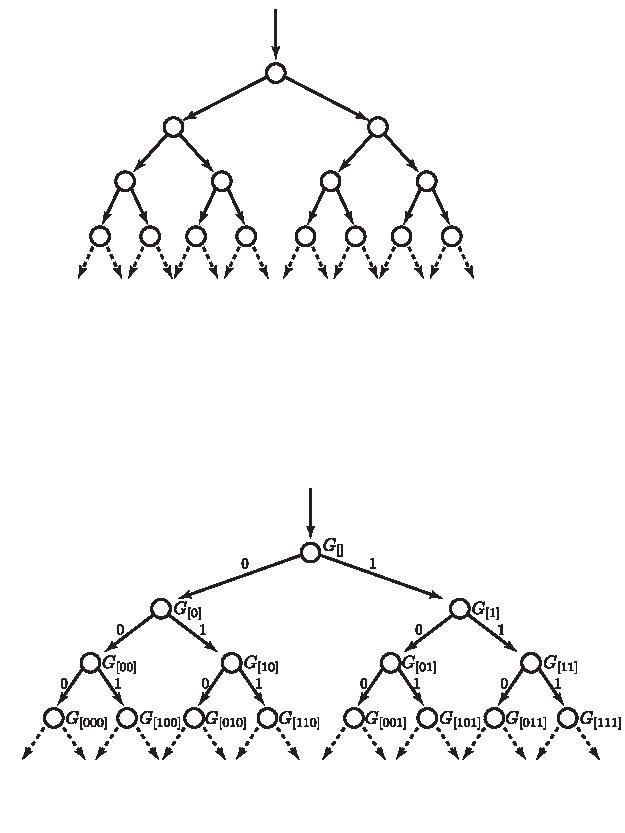
\includegraphics[trim = 2cm 2cm 2cm 10cm, width=8cm]{jtfig/base.pdf}
%\caption{Test perplexity vs.~number of training observations.}
\label{fig: gm_binary_complete}
\end{center}
\end{figure}
}


  \frame[t] {%slide 9
 \frametitle{Regularization}
 With Bayesian regularization we can do posterior inference of the following flavor
 
 \[P(x_{i+1} | \xbf_{1:i}) = \int G_{\xbf_{1:i}}(x_{i+1}) dP(G_{x_{i+1} }|\xbf_{1:i}) \]
 
 or more recognizably (but less accurately)
 
 \[P(x_{i+1} | \xbf_{1:i}) = \int P(x_{i+1} | \xbf_{1:i}, \GG) P(\GG | \xbf_{1:i}) d\GG \]

where, for DP's and PYP's we can represent and sample directly from $P(x_{i+1} | \xbf_{1:i})$ both individually and in hierarchies, leading to
 \[P(x_{i+1} | \xbf_{1:i}) \approx \sum_{\ell = 1}^L P(x_{i+1} | \xbf_{1:i}, \GG_\ell), \; \GG_\ell \sim P(\GG | \xbf_{1:i})\]

 }

  \frame[t] {%slide 27
 \frametitle{Binary Sequence Memoizer, \citet{Wood2009}}
\begin{eqnarray*}
\Sigma &=& \{0,1\}\\
\U_{\Sigma } &=& [.5, .5] \\
\\
	\G_{[]} | \U_{\Sigma}, d_0 &\sim& \PY(d_0, 0, \U_{\Sigma }) \\
		\G_{\bf{u}} | \G_{\sigma(\bf{u})}, d_{|\bf{u}|} &\sim& \PY(d_{|\bf{u}|}, 0, \G_{\sigma(\bf{u})}) \hspace{.35cm} \forall {\bf u} \in \Sigma^+\\
	x_n | x_{n-1},  \ldots, x_1 = \bf{u} &\sim& \G_{\bf{u}}
\end{eqnarray*}
Here $\sigma(x_1x_2x_3\ldots x_n) = x_2x_3\ldots x_n$ is the suffix operator.
\bigskip
\begin{center}
We're done, right?
\end{center}
}
\comment{
\begin{frame}[t]{Computational Problems}
\begin{itemize}
\item Number of nodes in graphical model is $\mathcal{O}(2^n)$
\begin{itemize}
\item Solution : marginalize (ignore) conditional distributions not found in sequence
\end{itemize}
\item Number of conditional distributions in graphical model still grows $\mathcal{O}(n^2)$
\begin{itemize}
\item Solution, \citet{Wood2009} : marginalize out non-branching nodes \cite{Pitman1999, Ho2006}
\item Use suffix tree algorithms to identify  $\mathcal{O}(n)$ remaining nodes.
\end{itemize}
\item Number of conditional distributions grows as $\mathcal{O}(n)$ but suffix tree algorithms require full sequence
\begin{itemize}
\item Solution, \citet{Gasthaus2010} : note (worst-case) $\mathcal{O}(n^2)$ inference time and show that incremental construction algorithm suffices
\end{itemize}
\item Number of nodes grows as $\mathcal{O}(n)$
\begin{itemize}
\item Solution, \citet{Bartlett2010} : forget nodes 
\end{itemize}
\end{itemize}
\end{frame}
}


\subsection{Sequence Memoizer}



 \begin{frame}[t]{Computational Problems}
\begin{itemize}
\item Number of nodes in graphical model is $\mathcal{O}(2^n)$
\begin{itemize}
\item Solution : marginalize (ignore) conditional distributions not found in sequence
\end{itemize}
\end{itemize}
\end{frame}
  
 
 
  \frame[t] {%slide 27
 \frametitle{Graphical Model}
 \begin{figure}[htbp]
\begin{center}
%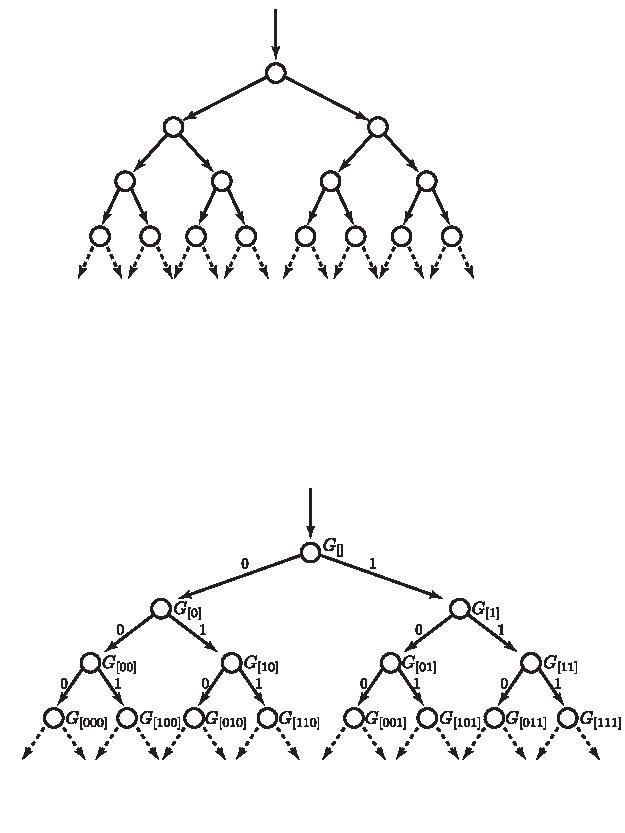
\includegraphics[trim = 4cm 8cm 4cm 8cm, clip, width=5cm]{jtfig/base.pdf}
\vspace{2cm}
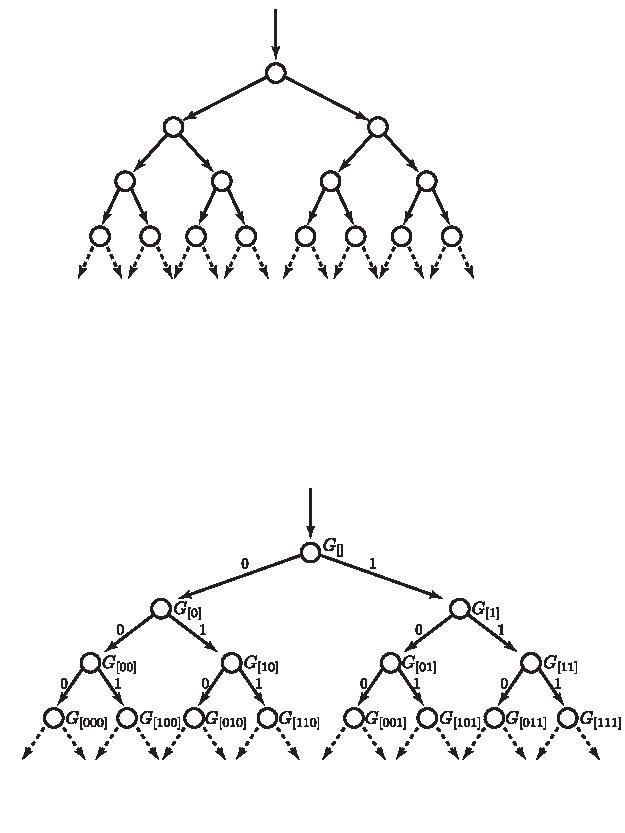
\includegraphics[trim = 2cm 2cm 2cm 10cm, width=8cm]{jtfig/base.pdf}
%\caption{Test perplexity vs.~number of training observations.}
\label{fig: gm_binary_complete}
\end{center}
\end{figure}
}

  \frame[t] {%slide 27
 \frametitle{110100, $G_{[]}(1)G_{[1]}(1)G_{[11]}(0)G_{[110]}(1)G_{[1101]}(0)G_{[11010]}(0)$}
 \begin{figure}[htbp]
\begin{center}
%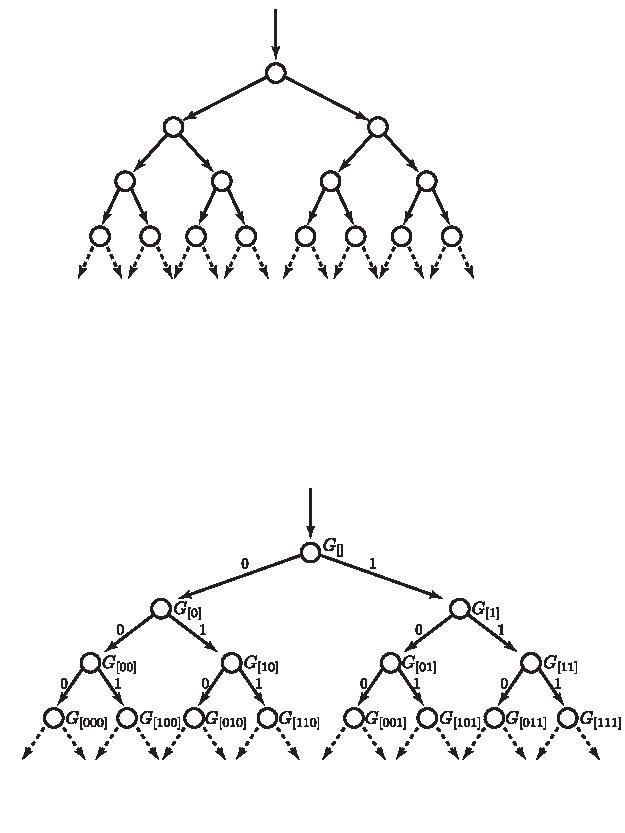
\includegraphics[trim = 4cm 8cm 4cm 8cm, clip, width=5cm]{jtfig/base.pdf}
\vspace{.42cm}
\hspace{.42cm}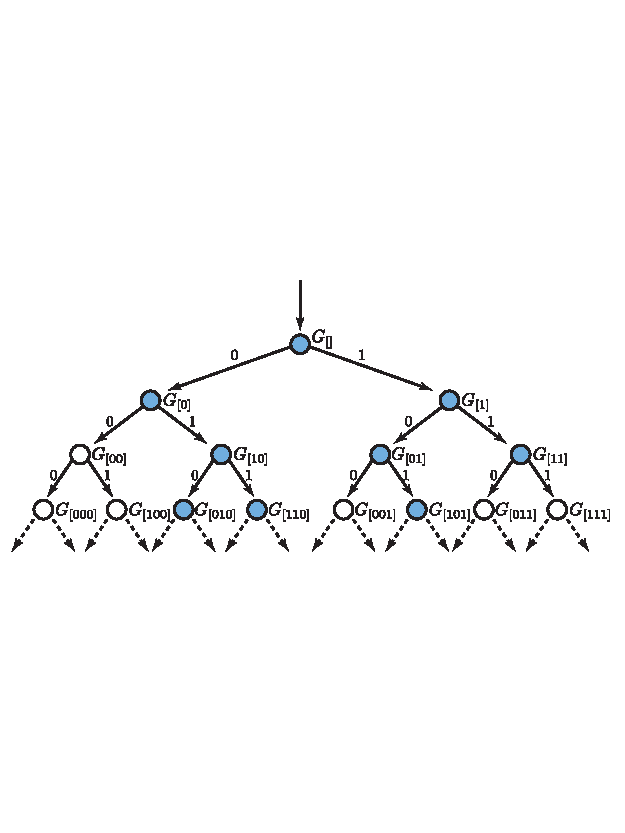
\includegraphics[trim = 2cm 2cm 2cm 5cm, width=8cm]{jtfig/base_color_2.pdf}
%\caption{Test perplexity vs.~number of training observations.}
\label{fig: gm_binary_complete}
\end{center}
\end{figure}
}

\begin{frame}[t]{Computational Problems}
\begin{itemize}
\item Number of nodes in graphical model is $\mathcal{O}(2^n)$
\begin{itemize}
\item Solution : marginalize (ignore) conditional distributions not found in sequence
\end{itemize}
\item Number of conditional distributions in graphical model still grows $\mathcal{O}(n^2)$
\begin{itemize}
\item Solution, \citet{Wood2009} : marginalize out non-branching nodes \cite{Pitman1999, Ho2006}
\item Use suffix tree algorithms to identify  $\mathcal{O}(n)$ remaining nodes.
\end{itemize}
\end{itemize}
\end{frame}



 \frame[t] {%slide 27
 \frametitle{Coagulation}
Consider a single path in the graphical model, say \[G_1\rightarrow G_2\rightarrow G_3\] with $G_2$ having no children other than $G_3$.    
\begin{block}{Theorem : Coagulation \cite{Pitman1999, Ho2006}}
If \[G_2| G_1\sim\py(d_1,0,G_1)\] and \[G_3| G_2\sim\py(d_2,0,G_2)\] then
\[G_3|G_1\sim\py(d_1d_2,0,G_1)\] with $G_2$ marginalized out.
\label{thm:coag}
\end{block}
Marginalizing out $G_2$ leaves $G_1\rightarrow G_3$ within the same PY family.

 }

 \frame[t] {%slide 27
 \frametitle{Graphical Model for 110100}
 \begin{figure}[htbp]
\begin{center}
%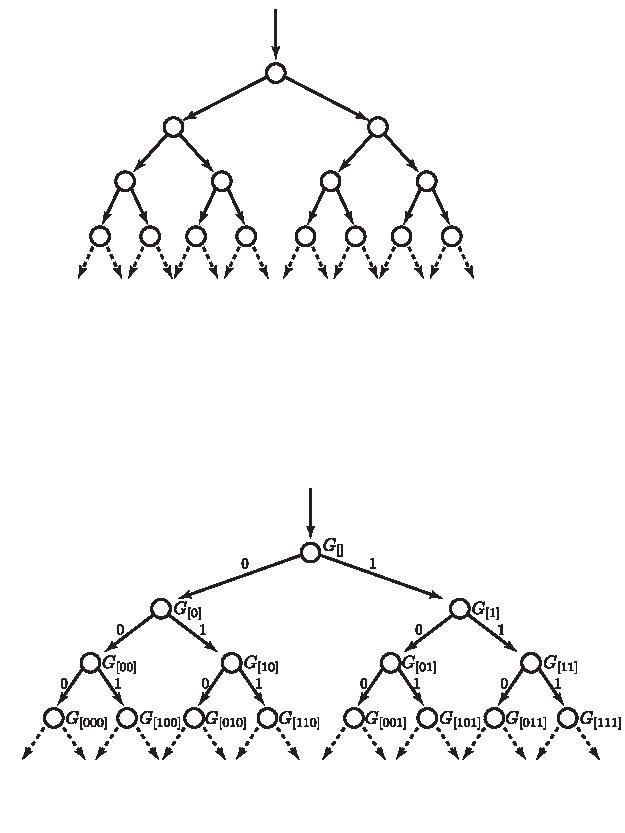
\includegraphics[trim = 4cm 8cm 4cm 8cm, clip, width=5cm]{jtfig/base.pdf}
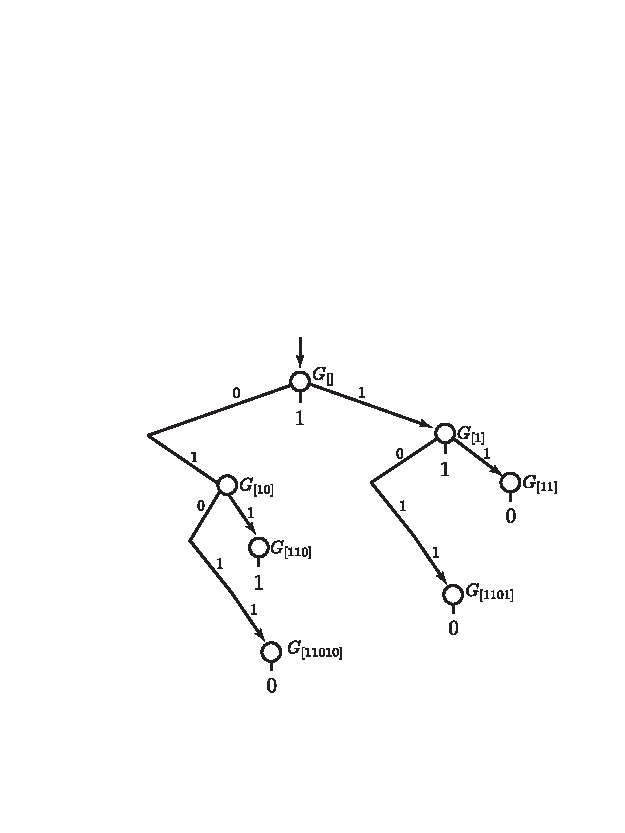
\includegraphics[trim = 2cm 2cm 2cm 6cm, width=8cm]{jtfig/seq_6.pdf}
%\caption{Test perplexity vs.~number of training observations.}
\label{fig: gm_binary_complete}
\end{center}
\end{figure}

 }

 \frame[t] {%slide 27
 \frametitle{Complete Graphical Model with 110100 Subset Highlighted}
 \begin{figure}[htbp]
\begin{center}
%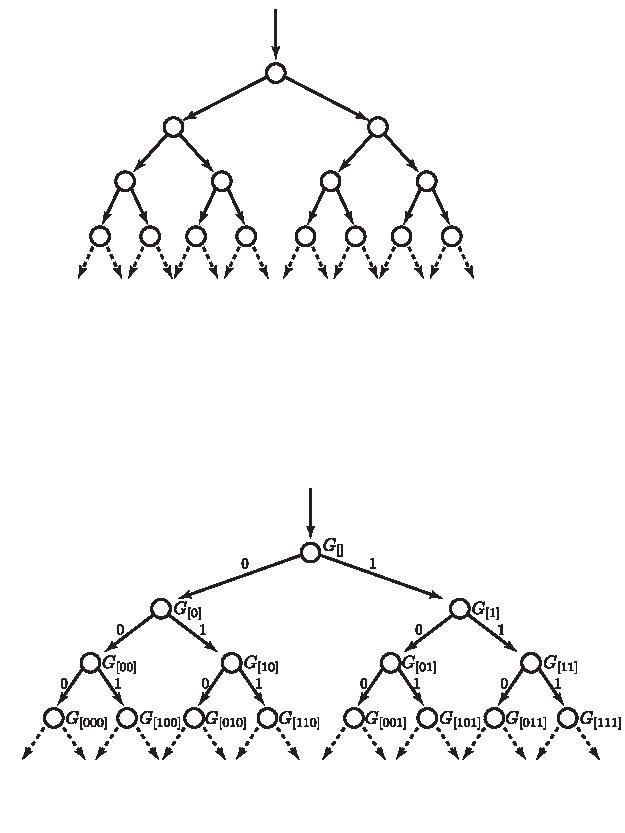
\includegraphics[trim = 4cm 8cm 4cm 8cm, clip, width=5cm]{jtfig/base.pdf}
\vspace{.42cm}
\hspace{.42cm}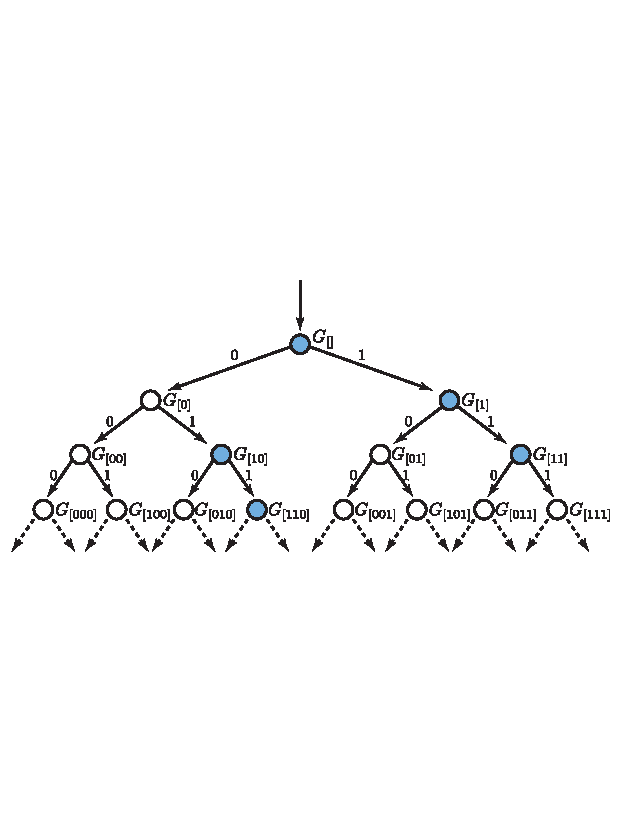
\includegraphics[trim = 2cm 2cm 2cm 5cm, width=8cm]{jtfig/base_color_1.pdf}
%\caption{Test perplexity vs.~number of training observations.}
\label{fig: gm_binary_complete}
\end{center}
\end{figure}
}

\begin{frame}[t]{Computational Problems}
\begin{itemize}
\item Number of nodes in graphical model is $\mathcal{O}(2^n)$
\begin{itemize}
\item Solution : marginalize (ignore) conditional distributions not found in sequence
\end{itemize}
\item Number of conditional distributions in graphical model still grows $\mathcal{O}(n^2)$
\begin{itemize}
\item Solution, \citet{Wood2009} : marginalize out non-branching nodes \cite{Pitman1999, Ho2006}
\item Use suffix tree algorithms to identify  $\mathcal{O}(n)$ remaining nodes.
\end{itemize}
\item Number of conditional distributions grows as $\mathcal{O}(n)$ but suffix tree algorithms require full sequence
\begin{itemize}
\item Solution, \citet{Gasthaus2010} : note (worst-case) $\mathcal{O}(n^2)$ inference time and show that incremental construction algorithm suffices
\end{itemize}
\end{itemize}
\end{frame}

  \frame[t] {%slide 27
 \frametitle{Graphical Model for 110100}
 \begin{figure}[htbp]
\begin{center}
%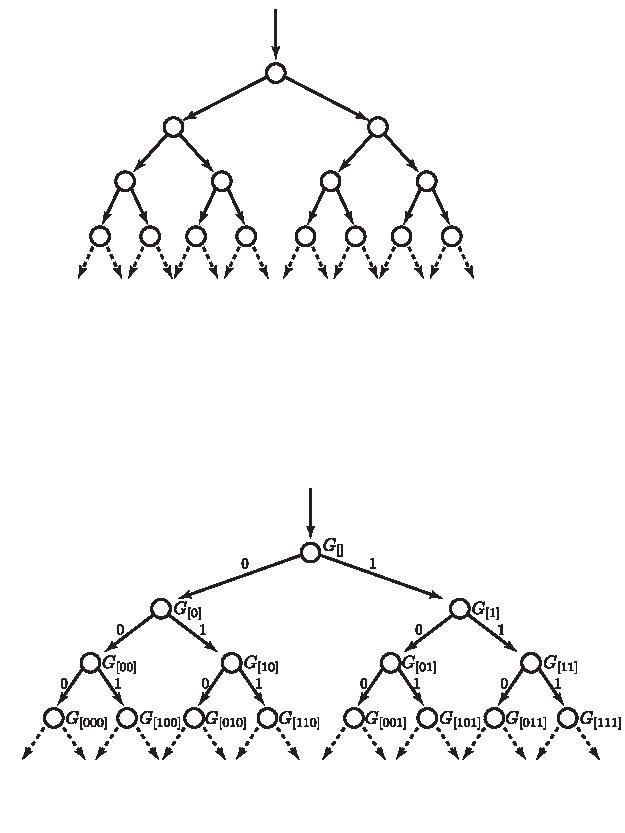
\includegraphics[trim = 4cm 8cm 4cm 8cm, clip, width=5cm]{jtfig/base.pdf}
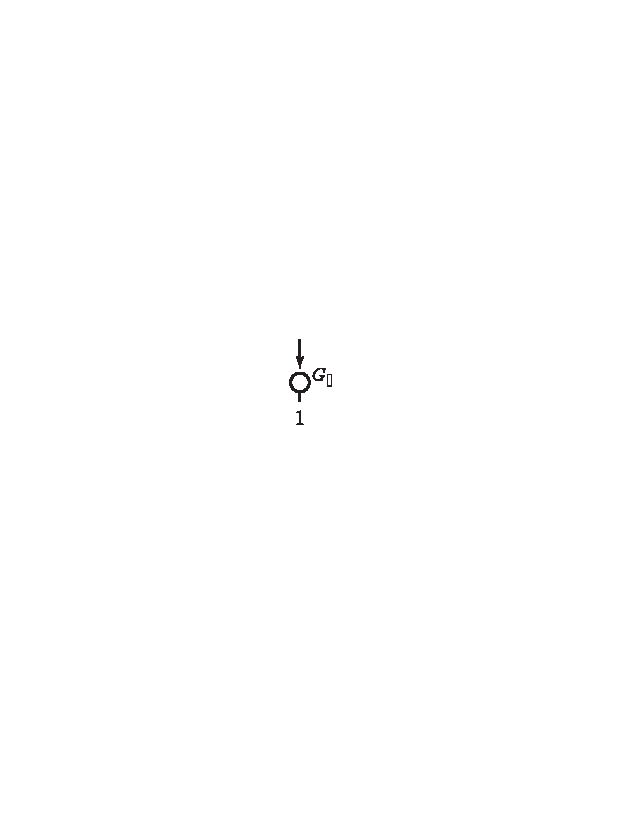
\includegraphics[trim = 2cm 2cm 2cm 6cm, width=8cm]{jtfig/seq_1.pdf}
%\caption{Test perplexity vs.~number of training observations.}
\label{fig: gm_binary_complete}
\end{center}
\end{figure}

 }
 
   \frame[t] {%slide 27
 \frametitle{Graphical Model for 110100}
 \begin{figure}[htbp]
\begin{center}
%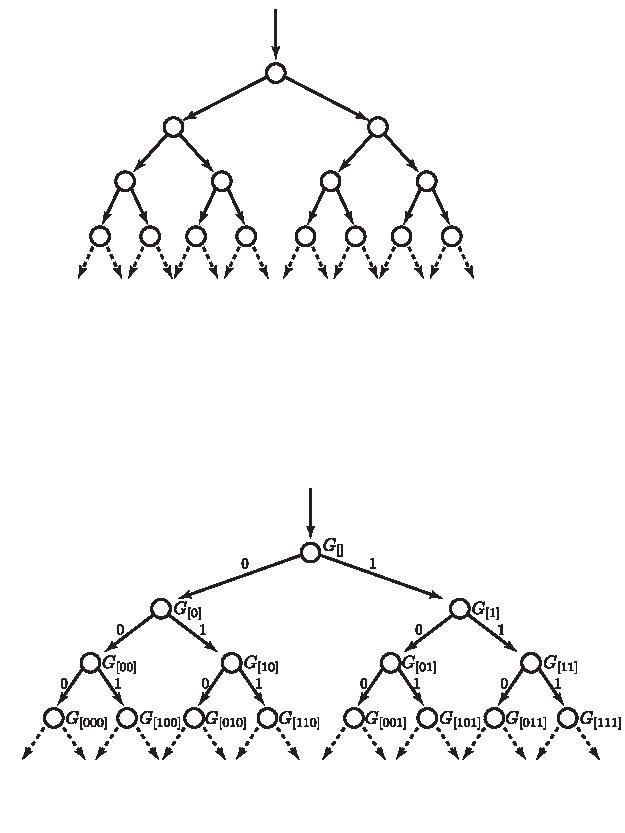
\includegraphics[trim = 4cm 8cm 4cm 8cm, clip, width=5cm]{jtfig/base.pdf}
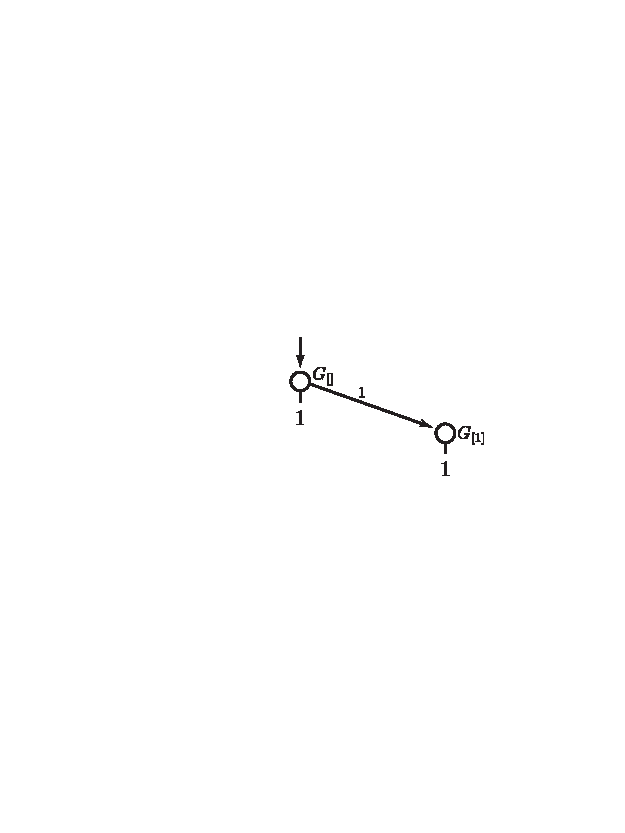
\includegraphics[trim = 2cm 2cm 2cm 6cm, width=8cm]{jtfig/seq_2.pdf}
%\caption{Test perplexity vs.~number of training observations.}
\label{fig: gm_binary_complete}
\end{center}
\end{figure}

 }

  \frame[t] {%slide 27
 \frametitle{Graphical Model for 110100}
 \begin{figure}[htbp]
\begin{center}
%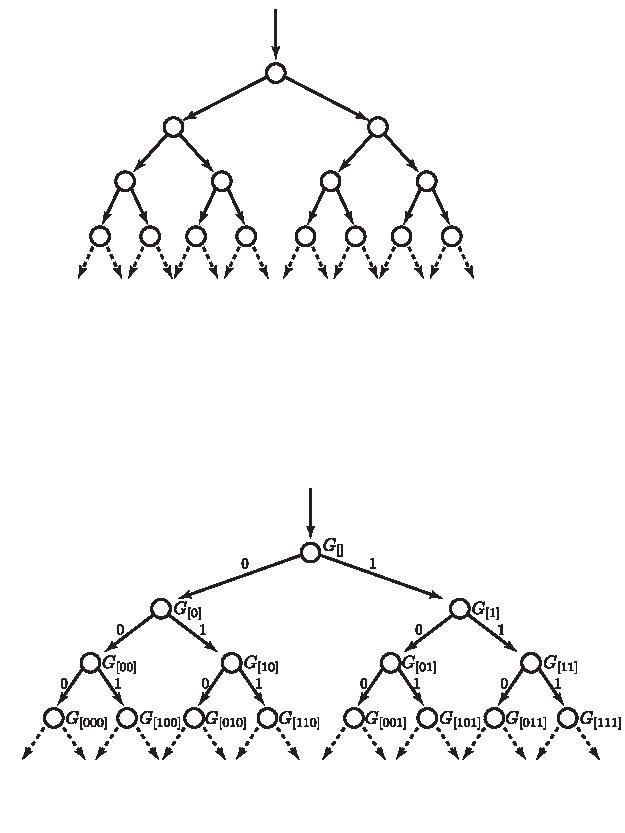
\includegraphics[trim = 4cm 8cm 4cm 8cm, clip, width=5cm]{jtfig/base.pdf}
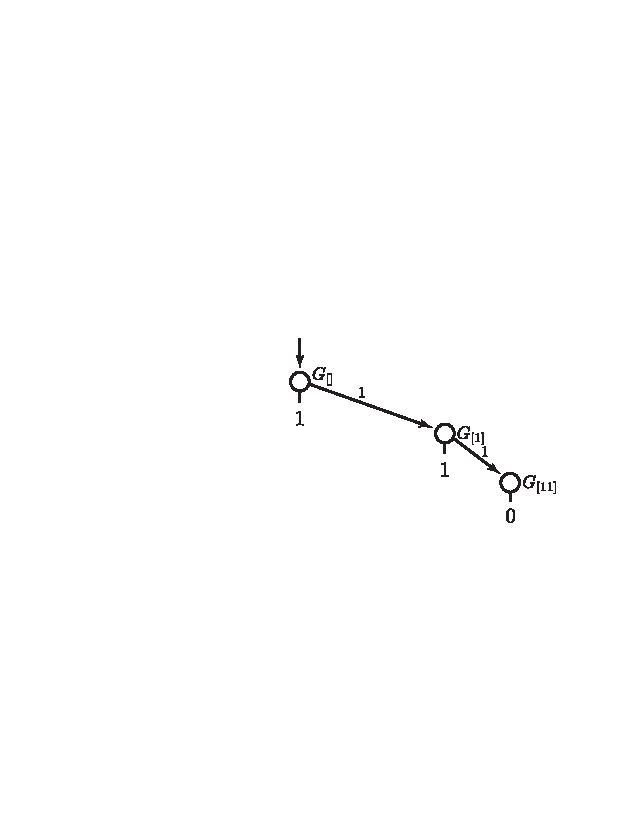
\includegraphics[trim = 2cm 2cm 2cm 6cm, width=8cm]{jtfig/seq_3.pdf}
%\caption{Test perplexity vs.~number of training observations.}
\label{fig: gm_binary_complete}
\end{center}
\end{figure}

 }
   \frame[t] {%slide 27
 \frametitle{Graphical Model for 110100}
 \begin{figure}[htbp]
\begin{center}
%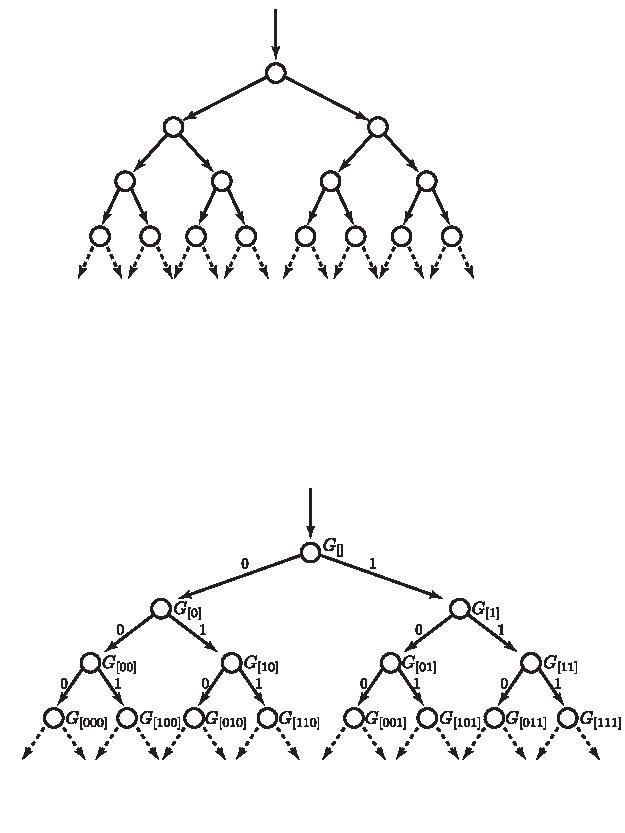
\includegraphics[trim = 4cm 8cm 4cm 8cm, clip, width=5cm]{jtfig/base.pdf}
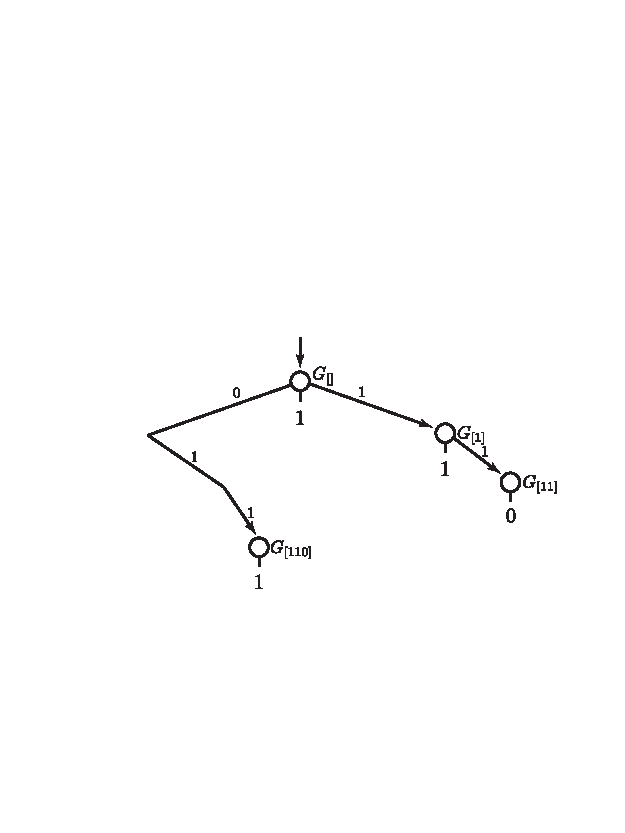
\includegraphics[trim = 2cm 2cm 2cm 6cm, width=8cm]{jtfig/seq_4.pdf}
%\caption{Test perplexity vs.~number of training observations.}
\label{fig: gm_binary_complete}
\end{center}
\end{figure}

 }
   \frame[t] {%slide 27
 \frametitle{Graphical Model for 110100}
 \begin{figure}[htbp]
\begin{center}
%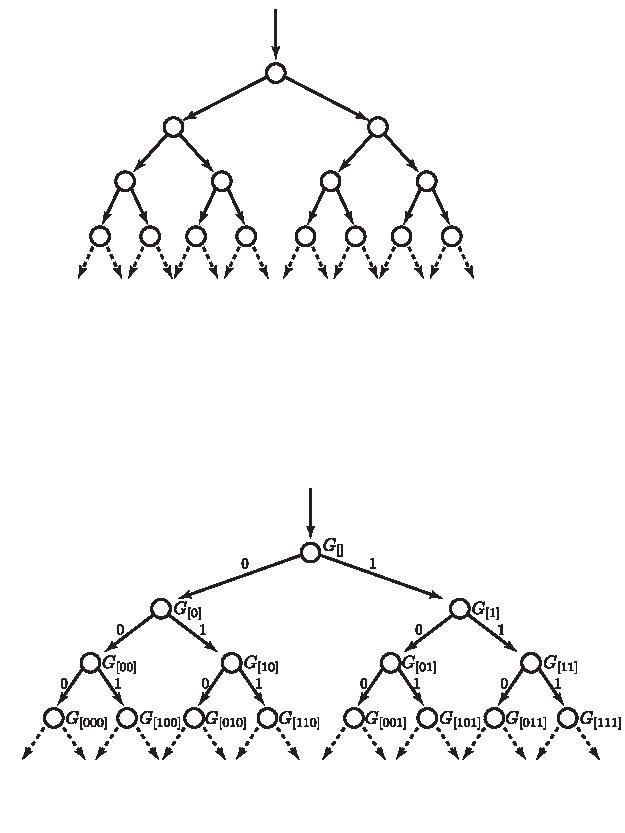
\includegraphics[trim = 4cm 8cm 4cm 8cm, clip, width=5cm]{jtfig/base.pdf}
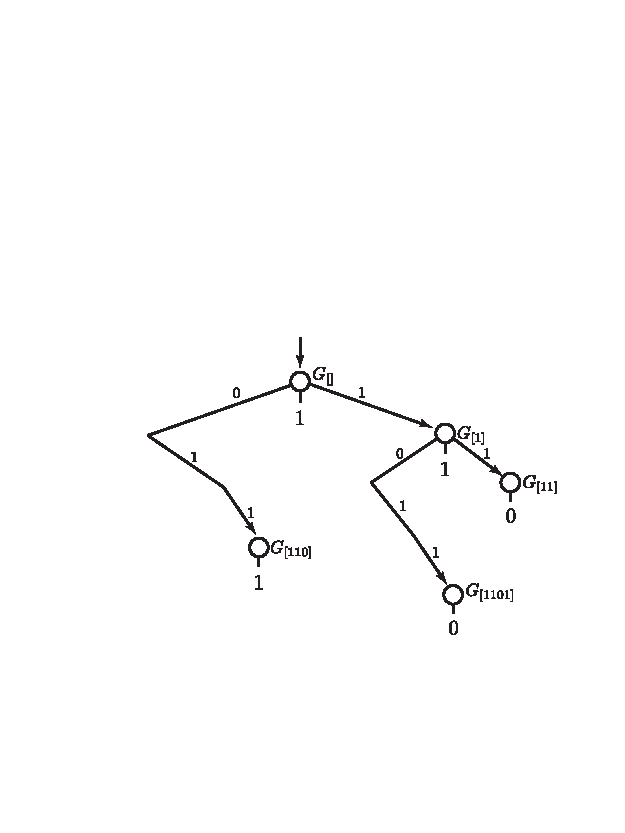
\includegraphics[trim = 2cm 2cm 2cm 6cm, width=8cm]{jtfig/seq_5.pdf}
%\caption{Test perplexity vs.~number of training observations.}
\label{fig: gm_binary_complete}
\end{center}
\end{figure}

 }
   \frame[t] {%slide 27
 \frametitle{Graphical Model for 110100}
 \begin{figure}[htbp]
\begin{center}
%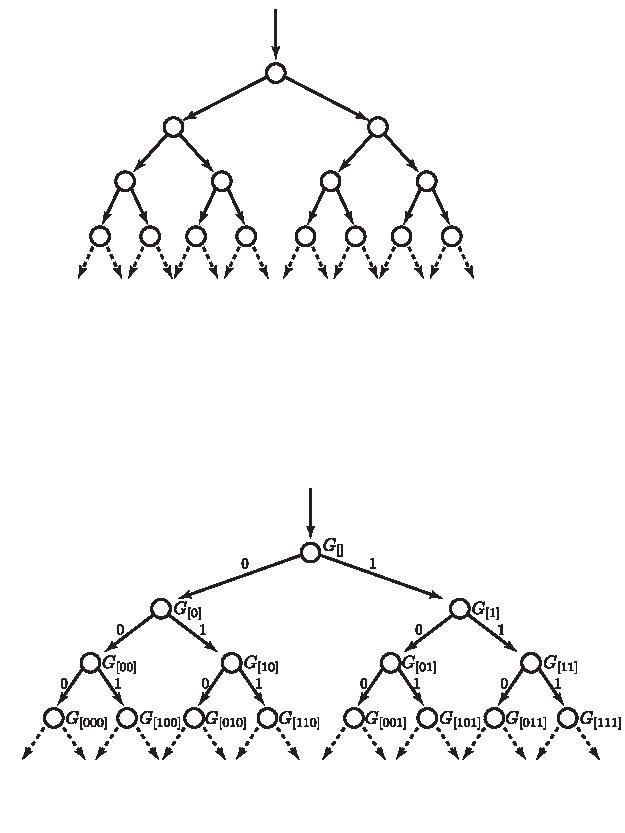
\includegraphics[trim = 4cm 8cm 4cm 8cm, clip, width=5cm]{jtfig/base.pdf}
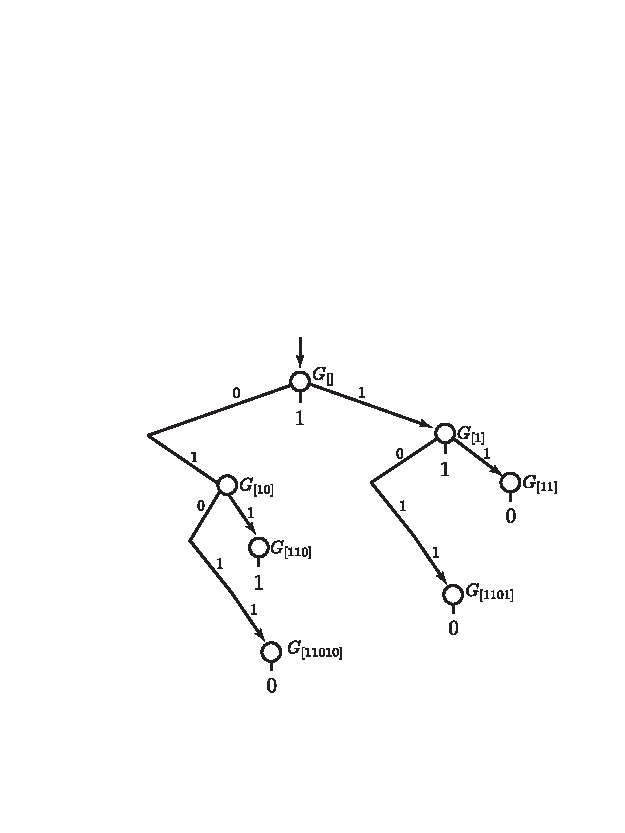
\includegraphics[trim = 2cm 2cm 2cm 6cm, width=8cm]{jtfig/seq_6.pdf}
%\caption{Test perplexity vs.~number of training observations.}
\label{fig: gm_binary_complete}
\end{center}
\end{figure}

 }
 
 \begin{frame}[t]{Computational Problems}
\begin{itemize}
\item Number of nodes in graphical model is $\mathcal{O}(2^n)$
\begin{itemize}
\item Solution : marginalize (ignore) conditional distributions not found in sequence
\end{itemize}
\item Number of conditional distributions in graphical model still grows $\mathcal{O}(n^2)$
\begin{itemize}
\item Solution, \citet{Wood2009} : marginalize out non-branching nodes \cite{Pitman1999, Ho2006}
\item Use suffix tree algorithms to identify  $\mathcal{O}(n)$ remaining nodes.
\end{itemize}
\item Number of conditional distributions grows as $\mathcal{O}(n)$ but suffix tree algorithms require full sequence
\begin{itemize}
\item Solution, \citet{Gasthaus2010} : note (worst-case) $\mathcal{O}(n^2)$ inference time and show that incremental construction algorithm suffices
\end{itemize}
\item Number of nodes grows as $\mathcal{O}(n)$
\begin{itemize}
\item Solution, \citet{Bartlett2010} : forget nodes 
\end{itemize}
\end{itemize}
\end{frame}

 \frame[t] {%slide 24
 \frametitle{Forgetting}
\begin{itemize}
\item Unit of memory is node in graphical model.  
\item Randomly removing leaf nodes defines a ``dependent hierarchical Pitman Yor process'' 
\item Incremental inference in this model is possible
\item The resulting model has constant storage complexity.
\end{itemize}
 }

 
 
 
